\section{Performance Evaluation}
We consider a $500 \times 500 m^2$ sparse sensing field with
$50-100$ relay nodes.
The Poisson-contact
mobility model is quasi-synthetic,
in which the parameter $\lambda$ is set to ?.
The speed of nodes is randomly selected in a uniform distribution changing from ? to ? m/s,
and the communication range of
these nodes is set to be ? m.
The parameter $\alpha$ is limited, i.e.,
$\alpha \in [0, 1]$.
we consider two cases in the simulations.
In the first case (Case 1),
we set ?.
in Case 2,
the contact rate
is ?.
In each simulation,
$M$ messages are created, 
whose maximal lifetime $T_m$ increases from $0$ to ? $s$.
Note that, 
all statistical results of our scheme are obtained by
repeating 50 times.

\subsection{Efficacy of the ODE model}
\label{subsec:pe_valid}
\begin{figure}
  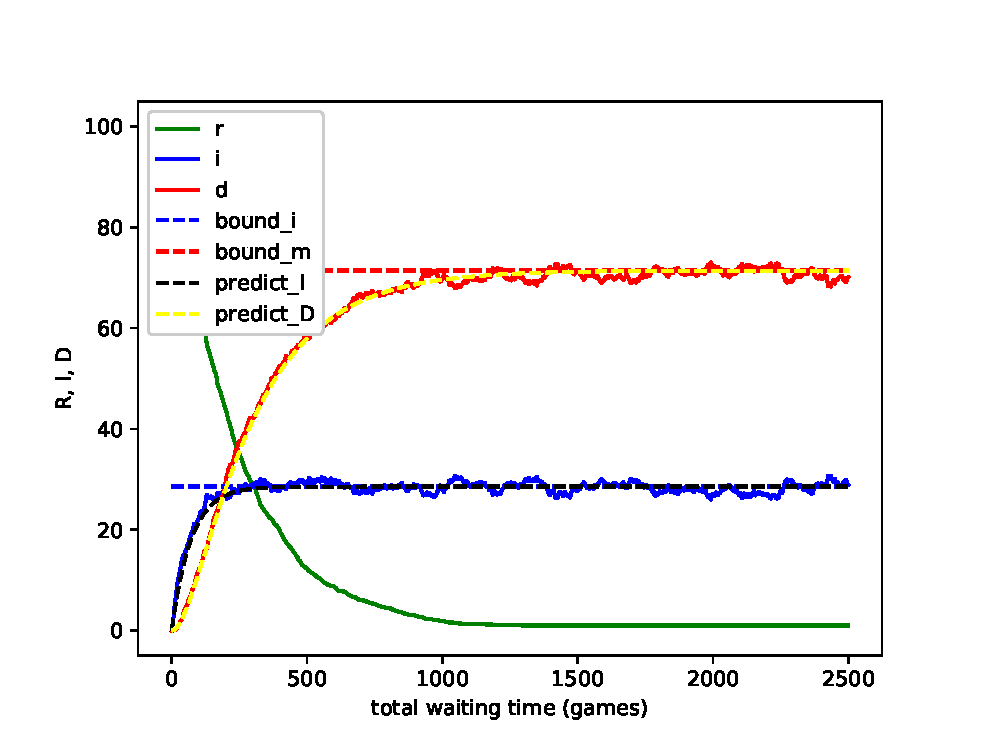
\includegraphics[width=.45\textwidth]{fig/twohop_without_detection.eps}
  \caption{$I(t)$, $D(t)$ and $R(t)$ with time $t$ computed from prediction and simulations
  when $\lambda = 0.004$, $\rho = 0.01$, $N=100$ and $T=2,500$.}
  \label{fig:twohop_predict_wod}
\end{figure}
Fig.~\ref{fig:twohop_predict_wod} shows that the change of the states
in the experiments conforms to the solved solutions (\ref{eq:IDR_wo_solu}).
Here $D(t)$, $I(t)$ and $R(t)$ are the mean values
at the specific time $t$ of $20$ simulations.
We can see from the figure that the $R,I,D$ with
The change of the states
in the experiments conforms to
the solved solutions.

[*** add $R(t)$ ***]
[*** add J P p ***]

\subsection{Efficacy of the approximate method}
\begin{figure}
  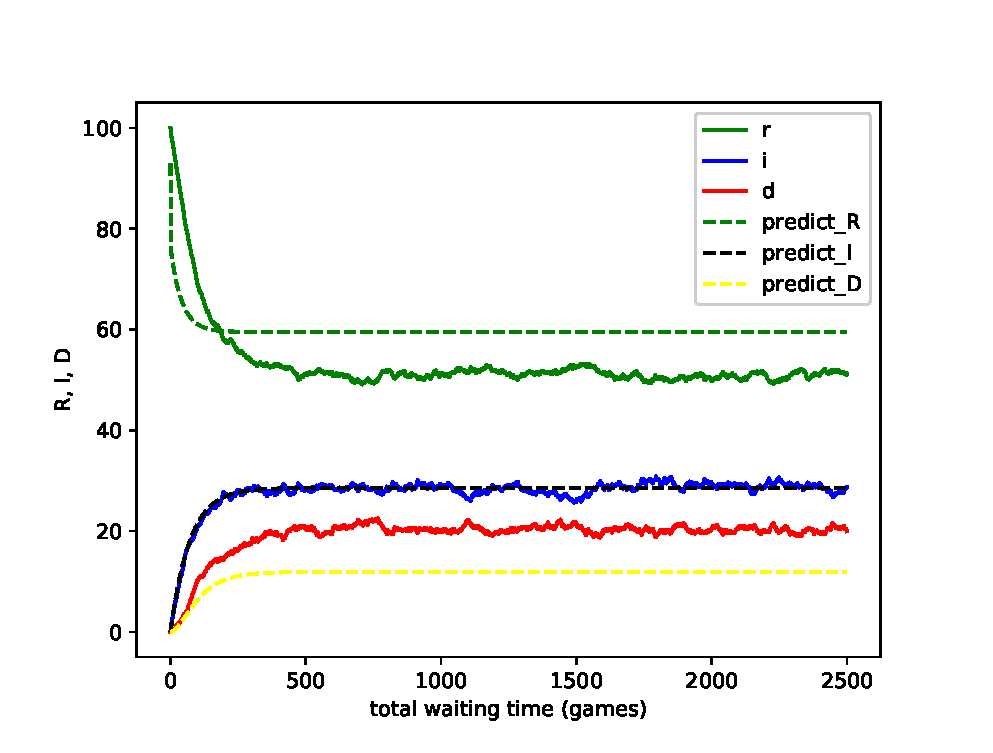
\includegraphics[width=.45\textwidth]{fig/twohop_with_fully_detection.eps}
  \caption{$I(t)$, $D(t)$ and $R(t)$ with time computed from prediction and simulations when $\lambda = 0.004$, $\rho = 0.011$, $N=100$,
  $T_{m} = 1$ and $T=2,500$.}
  \label{fig:twohop_predict_full_d}
\end{figure}
Fig.~\ref{fig:twohop_predict_full_d} shows (\ref{eq:IDR_full}).

\subsection{Optimal solution of selfish detection}
\begin{figure}
  \centering
  {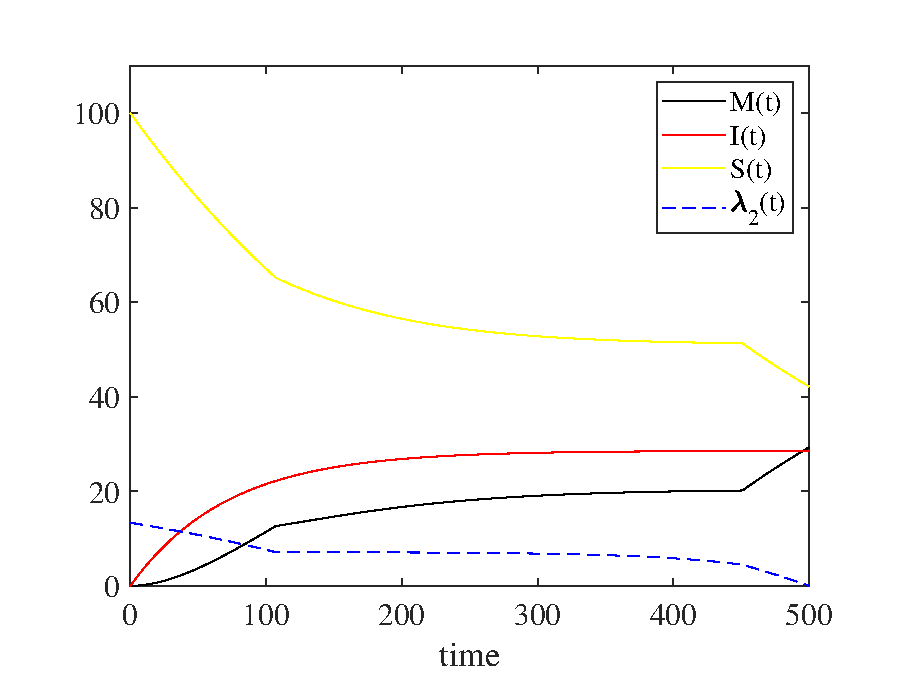
\includegraphics[width=0.47\textwidth]{fig/state.eps}}
     \caption{State variable of analysis with time.}
     \label{fig:pe_opt_state_time}
\end{figure}
\begin{figure}
  \centering
  {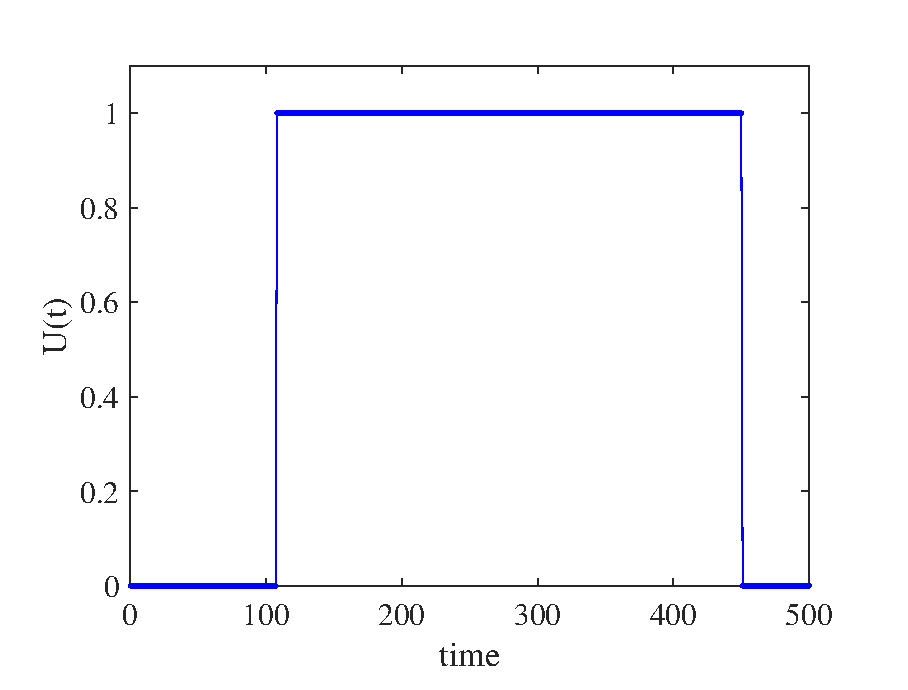
\includegraphics[width=0.47\textwidth]{fig/Ut.eps}}
     \caption{Control variable of analysis with time.}
     \label{fig:pe_opt_control_Ut}
\end{figure}
\begin{figure}
  \centering
  {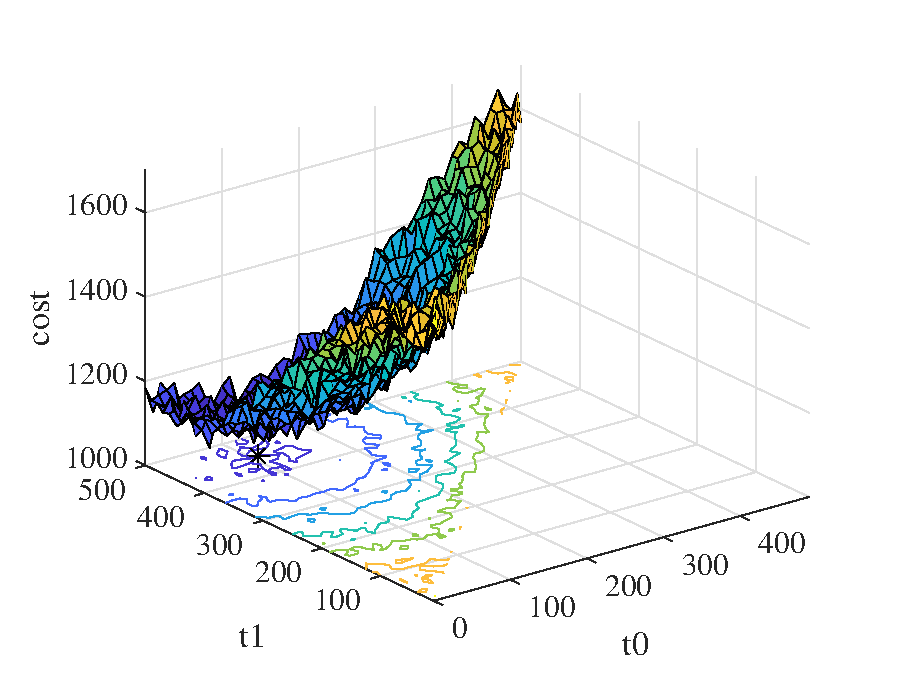
\includegraphics[width=0.47\textwidth]{fig/cost_all_t0t1.eps}}
     \caption{Different choices of $t0$ and $t1$.}
     \label{fig:pe_diff_choices}
\end{figure}
